I conducted an exploration and preprocessing of textual data, dividing it into a training set and a test set. I examined basic descriptive statistics regarding the length of the news articles. The average text length is approximately 80. Less than 25\% of the texts are longer than 100. This is significant because the maximum text length that can be used as input for BERT is 512. Therefore, text lengths should not pose a problem. In the case of texts longer than 512, they are truncated to a length of 512, and the remaining words are disregarded. It is also worth noting that the training set and the test set exhibit very similar statistics.

\begin{table}[!htbp]
\centering
{
\makegapedcells
\begin{tabular}{l|ll}
Statistics & Train set & Test set \\ \hline
Count & 11524 & 1267 \\ 
Mean  & 81   & 83  \\ 
Std   & 47    & 83   \\
Min   & 8    & 9   \\
25\%  & 56    & 57   \\
50\%  & 75    & 75   \\
75\%  & 100   & 99  \\
Max   & 2711  & 2560
\end{tabular}
}
\caption{Text length exploration}
\label{text_length}
\end{table}

Before merging multiple classes into two classes (for fake news and true news), I examined the cardinality of each individual class in order to combine them in a manner that would create a balanced binary class.

\begin{table}[!htbp]
\centering
{
\makegapedcells
\begin{tabular}{l|ll}
Class & Size \\ \hline
half-true   & 2362 \\
false       & 2258 \\
mostly-true & 2213 \\
barely-true & 1891 \\
true        & 1845 \\
pants-fire  & 955 
\end{tabular}
}
\caption{Class size before combining into two classes}
\label{class_size}
\end{table}

After the merger, the balance of both classes is represented as follows. The dataset balance is highly similar between the training and testing sets.

\begin{figure}[H]
\centering
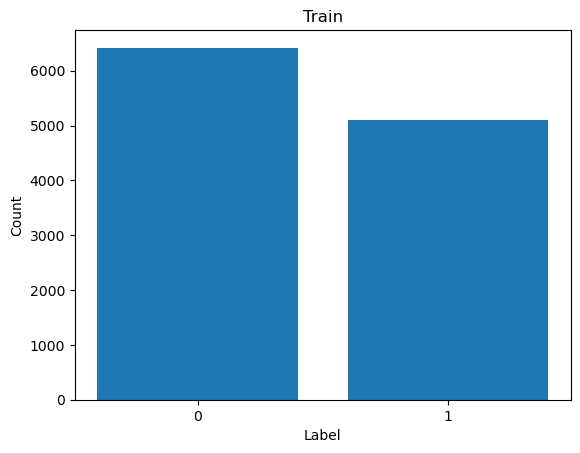
\includegraphics[width=0.7\linewidth]{train_balance.png}
\caption{Train set class balance}
\label{train_balance}
\end{figure}

\begin{figure}[H]
\centering
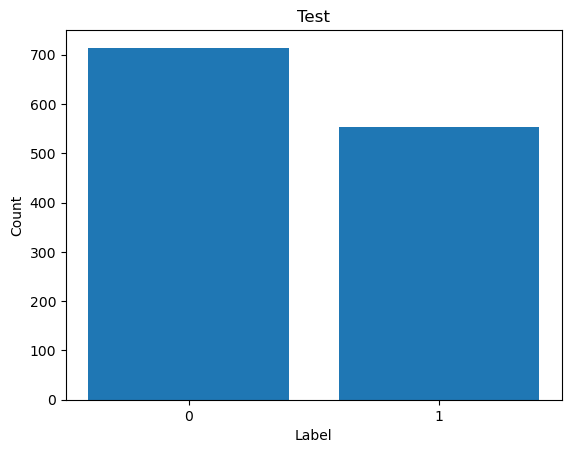
\includegraphics[width=0.7\linewidth]{test_balance.png}
\caption{Test set class balance}
\label{test_balance}
\end{figure}

Below are the wordclouds illustrating the frequency of words in the training and testing datasets.

\begin{figure}[H]
\centering
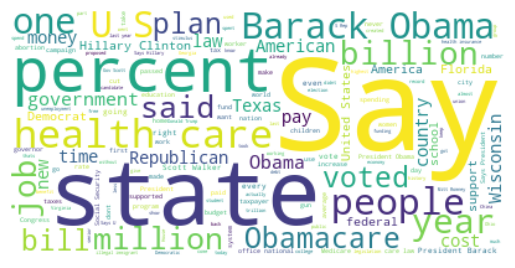
\includegraphics[width=0.7\linewidth]{wordcloud_train_fake.png}
\caption{Cloud of words of fake news in training set}
\label{wordcloud_train_fake}
\end{figure}

\begin{figure}[H]
\centering
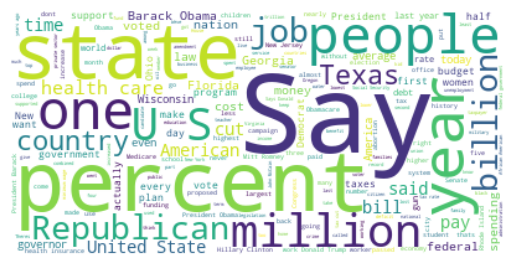
\includegraphics[width=0.7\linewidth]{wordcloud_train_true.png}
\caption{Cloud of words of true news for training set}
\label{wordcloud_train_true}
\end{figure}

\begin{figure}[H]
\centering
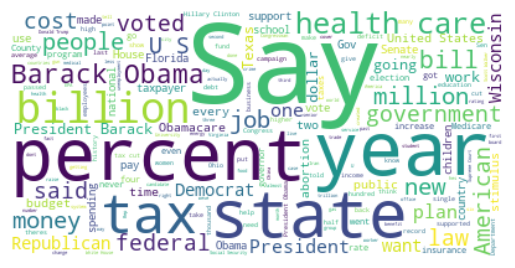
\includegraphics[width=0.7\linewidth]{wordcloud_test_fake.png}
\caption{Cloud of words of fake news for testing set}
\label{wordcloud_test_fake}
\end{figure}

\begin{figure}[H]
\centering
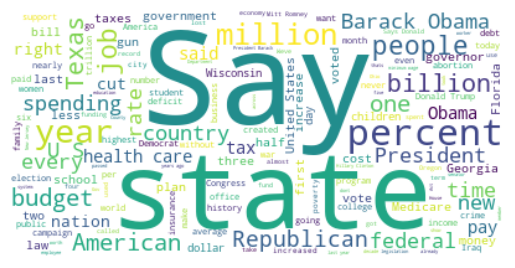
\includegraphics[width=0.7\linewidth]{wordcloud_test_true.png}
\caption{Cloud of words of true news for testing set}
\label{wordcloud_test_true}
\end{figure}